
	\section{Kurzfassung}
		
		Der erste Versuch beschäftigt sich mit der Elastizität von Stäben verschiedener Materialien. Das Ziel dieses Versuchs sind Elastizitätsmoduln\footnote{Plural von \glqq der Elastizitätsmodul\grqq {} nach Duden} für die verwendeten Materialien, welche mit den Literaturwerten übereinstimmen. Dazu werden an die eingespannten Stäbe Gewichte gehangen und die Auslenkung gemessen. Daraus und den Maßen der Stäbe wird dann der Elastizitätsmodul des jeweiligen Materials ermittelt. Die Ergebnisse dieses Versuchs %TODO
	
	\section*{drüber}
	
		Es wird angenommen, dass die Literaturwerte für den Elastizitätsmodul stimmen. Zur Überprüfung dieser Hypothese dient der folgende Versuch.		
		
	\section{Methoden}
		
		\subsection*{Aufbau}
		Der Aufbau dieses Versuches ist in Abb. \ref{abb:linearerFit} dargestellt. Hierbei werden Stäbe aus verschiedenen Materialien eingespannt und deren Auslenkung beim Anhängen eines Gewichtes gemessen. 
		Die verwendeten Materialien wurden durch ihre Farbe und ihr Gewicht bestimmt. Es handelt sich um runde Stäbe aus Messing, Stahl und Aluminium. Zusätzlich wird ein quaderförmiger Stab aus Messing untersucht, um zu betrachten, wie sich dieser hoch- bzw. flachkant eingespannt verhält.
		
		Mit Hilfe eines Maßbandes werden die Längen der Stäbe gemessen und mit einer Mikrometerschraube deren Breiten. Um zu prüfen, ob die Stäbe an jeder Stelle die gleiche Breite besitzen, wird die Breitenmessung an fünf Stellen jeweils drei mal durchgeführt, da die Mikrometerschraube verschiedene Werte misst, je nachdem wie stark geschraubt wird. 
		Für die Messung werden pro Stab jeweils fünf verschiedene Gewichte angehängt und die Auslenkung dabei an einem Maß auf einem Spiegel parallaxenfrei abgelesen. Zur Bestimmung dieser Auslenkung, wird der Wert für die Ruhelage (bei $m=\SI{0}{\g}$) gemessen und von dem gemessenen Wert bei angehängter Masse unterschieden. Für jedes neue Gewicht wird der Wert für die Ruhelage neu bestimmt, um mögliche Ungenauigkeiten, wie durch leichte Verbiegungen des Stabes, zu vermeiden.
		
		\subsection*{Unsicherheiten}
		Für die Unsicherheiten bei den Längenmessungen werden Dreiecksverteilungen verwendet. Bei der Mikrometerschraube lassen sich die Werte auf \SI{0,01}{\mm} genau ablesen, dies wird für die Verteilung verwendet. Für das Maßband und das Maß auf dem Spiegel ergibt sich dieselbe Unsicherheit, da bei beiden das Ablesen auf \SI{1}{\mm} genau möglich war.
		Die Massen waren gegeben und werden als absolut angesehen. Hier treten demnach keine Unsicherheiten auf.	
	\section{Messung}
		
		Die Messung der Länge der Stäbe ergab die in Tab. \ref{tab:Stablängen} gelisteten Werte. Hierbei wurde bei allen Stäben der Einspann von \SI{2+-0,122}{\cm} abgezogen und die Unsicherheiten kombiniert.
		\begin{table}[h]
			\caption{Länge der Stäbe}
			\centering
			\label{tab:Stablängen}
			\begin{tabular}{c|c}
				{Material} & {Länge}\\
				\hline
				{Messing (eckig)} & \SI{29,2+-0,173}{\cm}\\
				{Messing (rund)} &  \SI{29,2+-0,173}{\cm}\\
				{Stahl} & \SI{28,9+-0,173}{\cm}\\
				{Aluminium} & \SI{28,6+-0,173}{\cm}\\		
			\end{tabular}
		\end{table}
	
		Für die Breite der Stäbe sind die gemittelten Werte für die verschiedenen Messpunkte in Tab. \ref{tab:Stabbreiten} angegeben. Auch hier ergibt sich  eine kombinierte Unsicherheit.
		\begin{table}[h]
			\caption{Breite der Stäbe}
			\centering
			\label{tab:Stabbreiten}
			\begin{tabular}{c|c}
				{Material} & {Länge}\\
				\hline
				{Messing (eckig)} & \SI{29,2+-0,173}{\cm}\\
				{Messing (rund)} &  \SI{29,2+-0,173}{\cm}\\
				{Stahl} & \SI{28,9+-0,173}{\cm}\\
				{Aluminium} & \SI{28,6+-0,173}{\cm}\\		
			\end{tabular}
		\end{table}
		
		\begin{figure}[ht]
			\centering
			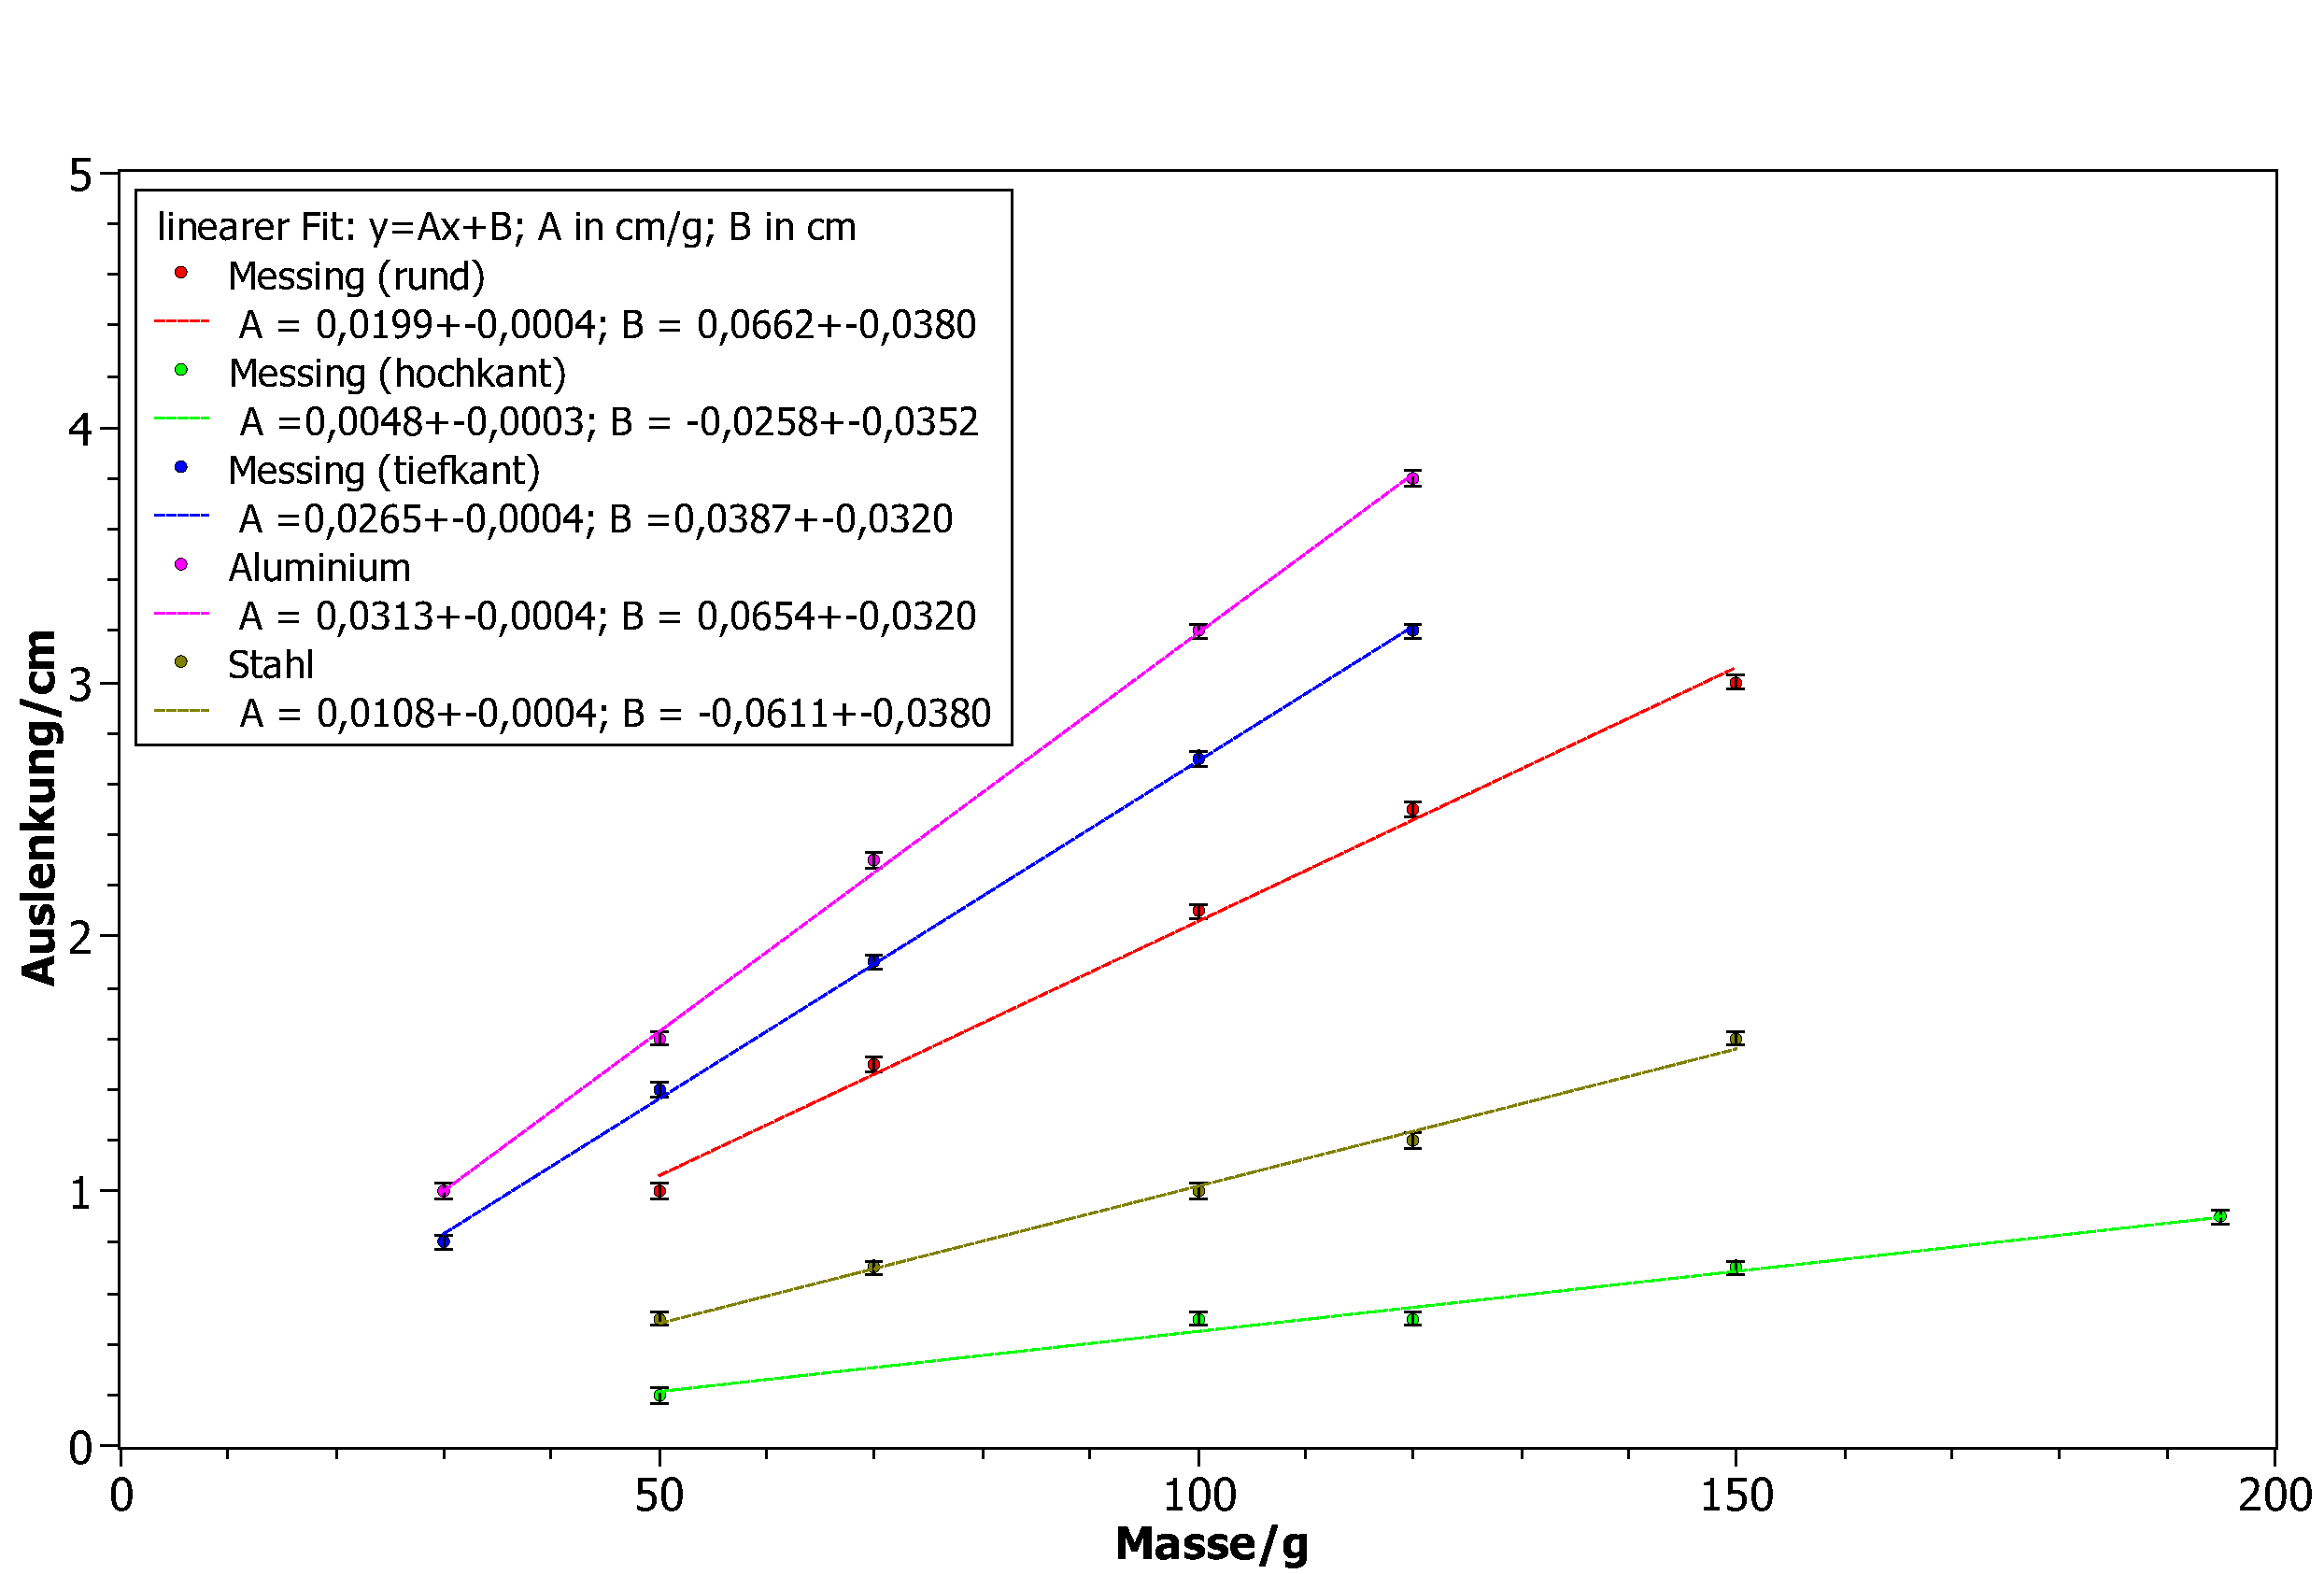
\includegraphics[width=\textwidth]{StabAuslenkungen.pdf}
			\caption{Auslenkung der Stäbe in Abhängigkeit der angehängten Masse}
			\label{abb:linearerFit}	
		\end{figure}
			
		\begin{figure}[ht]
			\centering
			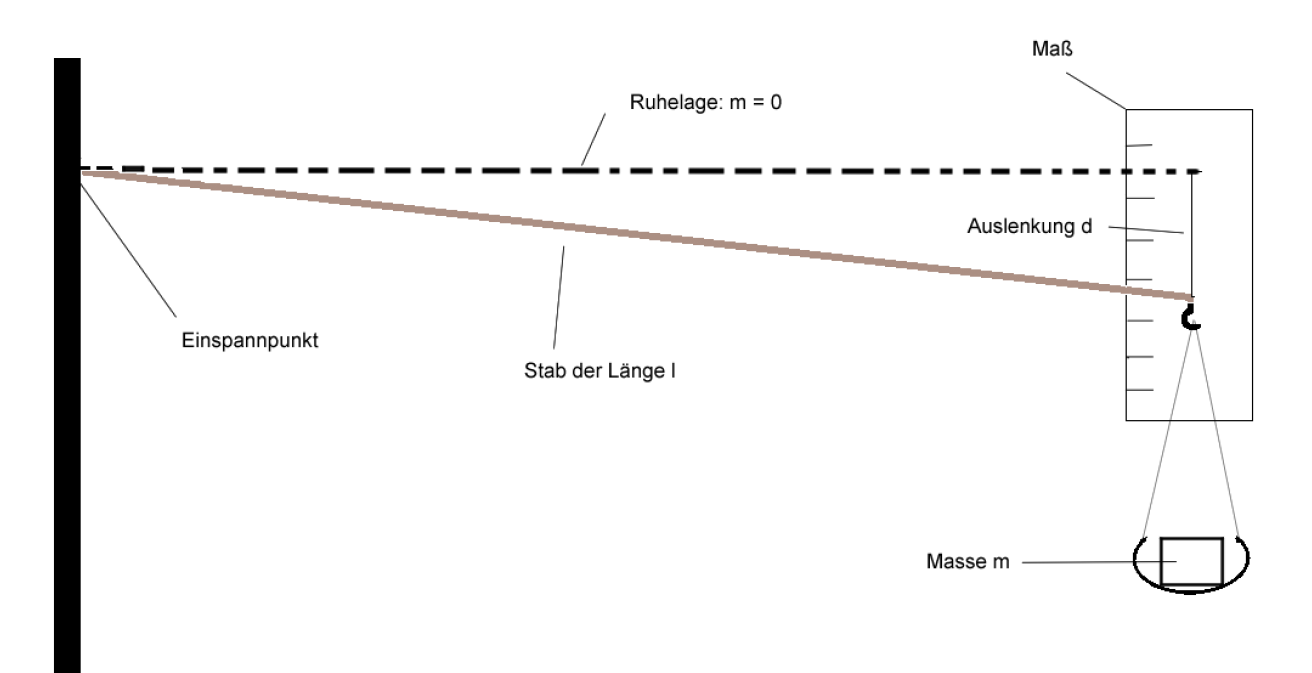
\includegraphics[width=\textwidth]{StabAuslenkungSkizze.png}
			\caption{Auslenkung der Stäbe in Abhängigkeit der angehängten Masse}
			\label{abb:2}	
		\end{figure}	
		
	\section{Diskussion}